---
id: tkz-euclide-ejemplo-50
title: "Transportador"
description: "Coloca un transportador en un vértice y dibuja los rayos que determinan el ángulo."
keywords: [transportador, angulo, rayos, medicion]
tags: [tkzProtractor]
sort: 50
---
\documentclass[tikz,border=2mm]{standalone}
\usepackage{tkz-base}
\usepackage{tkz-euclide}

\begin{document}
    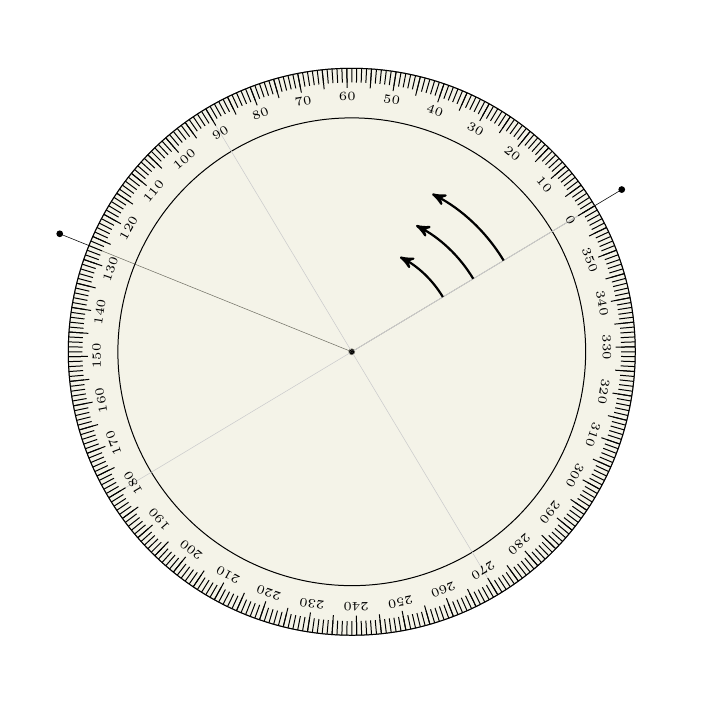
\begin{tikzpicture}
        % Define el vértice A y el origen O (opcional para referencia).
        \tkzDefPoint(2,0){A}
        \tkzDefPoint(0,0){O}
    
        % Define los puntos B y C a partir de A, usando dirección/longitud polar.
        \tkzDefShiftPoint[A](31:4){B}
        \tkzDefShiftPoint[A](158:4){C}
    
        % Dibuja los puntos y los rayos AB y AC (formando un ángulo en A).
        \tkzDrawPoints(A,B,C)
        \tkzDrawSegments(A,B A,C)
    
        % Coloca un transportador de ángulos en A orientado por AB.
        \tkzProtractor[scale=0.9](A,B)
    \end{tikzpicture}
\end{document}
